
% this file is called up by thesis.tex
% content in this file will be fed into the main document

%: ----------------------- introduction file header -----------------------
% the code below specifies where the figures are stored
\graphicspath{{3/figures/}}

\chapter{Deep Learning}
\label{chp:background}

% Goals
%  -

As with any work that suggests an alternate trajectory within a given field of study, it is necessary to not only understand the current state of affairs but also how it came to be.
Electrical engineering and computer science have now spent the better part of a century developing information processing systems under the banner of myriad titles and directions, and even a cursory review of both helps to further demonstrate the potential impact of this research.
This is followed by a formal definition of the modular components used in deep learning.
Once contextualized, recent advances in deep learning are addressed to showcase the advantages of these methods and how they can be extended to open problems in time-domain signal processing.


\section{Foundations of Information Processing}
\label{sec:foundations}

Due to advances in machine computation, there are primarily two different ways to conceptualize the design of information processing models relevant to the work proposed here.
One approach is based on signal theory as viewed through the lens of electrical engineering, whereas the other focuses on graphical models of artificial neural processing grounded in computer science.
Though broad topics of study in themselves, they are worth mentioning together for two crucial reasons: first, a majority of inertia developed within the field of MIR is due largely to its roots in the former; and second, it is a useful juxtaposition to form when marrying these disconnected topics.
%Electrical engineering formalized as a discipline in the middle of the $19^{th}$ century on the heels of inventions such as the telegraph and electric power distribution.
Much early work in electrical engineering stemmed from the realization that electricity could be used to represent measurable phenomena and therefore capture, store, and transmit this information.
These representations are referred to as analog signals because they use one representation---time-varying voltage, for example---to mirror another one---such as a sound pressure wave---in a continuous fashion.
It was soon discovered that not only could this information be represented via electricity, but that it was also possible to analyze and manipulate it for a variety of applications.
Heavily grounded in classic numerical analysis methods of the $17^{th}$ and $18^{th}$ centuries, these methods are referred to as signal processing.
Through experimentation in physics, scientists found that certain electromagnetic materials could be used to affect electricity in predictable ways, and when connected in an electrical circuit could be used to filter, or augment, signals.
%Any system can be uniquely characterized by how it responds to an instantaneous pulse of energy, known as an impulse response in time or transfer function in frequency.
%The properties of electric components were then formalized into similar mathematical expressions, giving rise to signal theory.
%This made it possible to express and design complex filters by analyzing the overall transfer function, so long as the derivation was tractable.
Importantly, the need to solve signal processing systems by inspection requires that the entire system be linear and time invariant (LTI), because the violation of either property makes mathematical analysis far too difficult, if not altogether impossible.

With the advent of solid-state transistors and subsequently computers in the mid-$20^{th}$, digital representations of signals could be produced by sampling analog waveforms to be manipulated numerically, referred to as digital signal processing (DSP).
Digital signals---those that also represent some kind of real world phenomena, at least---differ from analog ones in two important aspects: the signal takes values from a finite set of discrete numbers, and these quantities are measured at precise moments in time.
Therefore, digital signals are specified by a sequence of real-valued numbers $x[n]$, rather than a generated, continuous function $x(t)$.
When this transition to numerical computation began, the effort was made to reformulate previous knowledge regarding analog signal theory and processing into the digital domain.
Similar to those in analog theory, digital filters can be expressed explicitly by a transfer function, which can be translated directly to a set of coefficients representing the linear difference equation, generically given by the following:

\begin{equation}
\label{eq:diffeq}
\begin{array}{rcr}
y[n] & = & b_0x[n] + b_1x[n-1] + b_2x[n-2] + b_3x[n-3] \ldots \\
 & & - a_1y[n-1] - a_2y[n-2] - a_3y[n-3] \ldots
\end{array}
\end{equation}

There are typically said to be two categories of digital filters: Finite Impulse Response (FIR), or non-recursive, filters and Infinite Impulse Response (IIR), or recursive, filters.
As illustrated in Figure \ref{fig:filters}, an FIR filter is actually a special case of the more general IIR filter, where the feedback connections---the $a$-coefficients in Equation (\ref{eq:diffeq})---have all been set to zero.
Though digital filters are not constrained by the availability or precision of manufactured electrical components, they are still traditionally constrained to be LTI systems for the same reasons as their analog counterparts.
As a result, non-linear signal processing models in both the analog and digital domains are historically unpopular due to inherent challenges in the mathematical formulation.

\begin{figure}[!t]
\centering
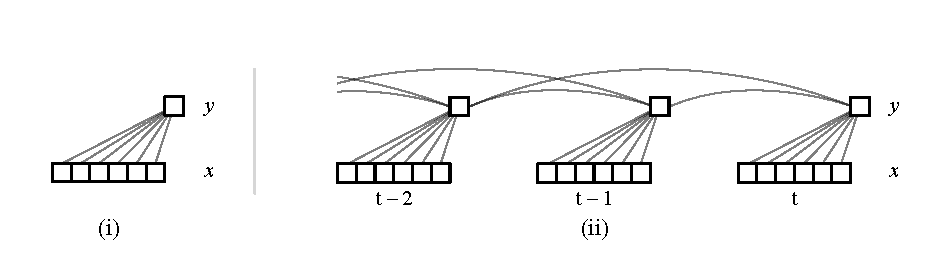
\includegraphics[width=\textwidth]{filters_2}
\caption{\small{Finite Impulse Response (i) and Infinite Impulse Response (ii) digital filters. Multiplication is shown along the edges of each connection.}}
\label{fig:filters}
\end{figure}

Slightly more recently, the field of computer science was established in the first half of 20th century, adapting the rules of Boolean logic to electrical switches and laying the groundwork for what would become the modern computer.
Developing a theory of computation, the discipline places a strong emphasis on the theory and design of machines that process and manipulate information.
In some cases, this can be considered AI, where the goal is to produce machines capable of performing at---or beyond---the capacity of a human expert.
Due in no small part to these ambitions, interest in neural computation arose from the desire to craft biologically plausible information processing machines.
One particular model of note is the Perceptron, a simple nonlinear model defined by the following:

\begin{equation}
\label{eq:perceptron}
f(x) = \begin{cases}1 & \text{if }w \cdot x + b > 0\\0 & \text{otherwise}\end{cases}
\end{equation}

Each output, for vectors $x$ and $w$ of equal length, is said to be a unit, and a matrix of $w$-coefficients will yield some number of parallel units.
However, as addressed by Minsky and Papert \cite{Minsky1969} in 1969, a single Perceptron could not implement the XOR function.
Seen as a fundamental deficiency, this and other similar criticisms led to a sharp decline in funding for neural network research.
It would later be discovered that the answer to this problem is to form a cascade of \emph{multiple} Perceptrons, and this very instance illustrates the case well.
Expressed symbolically, for two inputs $p$ and $q$, the XOR is defined as the composite of simpler operations:

\begin{equation}
\label{eq:xor}
p \oplus q = (p \wedge \neg q) \vee (\neg p \wedge q)
\end{equation}

\noindent While true that a single Perceptron cannot realize the complete logic expression of an XOR, it is integral to note that it \emph{can} produce either of the parenthetical statements.
Then, a third Perceptron can be used to form the disjunction of the two simpler statements, realizing the intended XOR function.

Extending beyond this toy example, neural networks can be conceptualized in the most general sense as an information processing system characterized by two qualities: an architectural design, or model, and a flexible parameterization that can be learned from data.
In practice, neural networks are not constrained to operate on binary logic values, but rather can be applied directly to digital signals in the domain that they are perceived by humans, e.g. the pixel values of an image.
Each layer in an architecture can be said to extract features that are useful for solving some task.
Ideally, these features are \emph{learned} automatically using what are known as gradient methods, the basic idea being that a function attempts to reduce how ``wrong'' it is by taking small steps toward better answers; by analogy, this is a bit like climbing down a mountain blind-folded.
For this to be possible, the activation of each node, as expressed in Equation (\ref{eq:perceptron}), must be softened such that the function is differentiable.
In the broadest sense, the two types of neural network architectures of interest here are fully-connected and recurrent networks, illustrated in Figure \ref{fig:networks}.
Both are historically applied to static, multidimensional inputs and often used to classify an observation.
An example use case would be providing several observed statistics about an organism to a network and attempting to determine its species.
If one of the input dimensions for this input is time, it is referred to as a Time-Delay Neural Network (TDNN).
Alternatively, a Recursive Neural Network (RNN) includes feedback connections between current output nodes in the hidden layer and the output nodes of the previous observation.

\begin{figure}[!t]
\centering
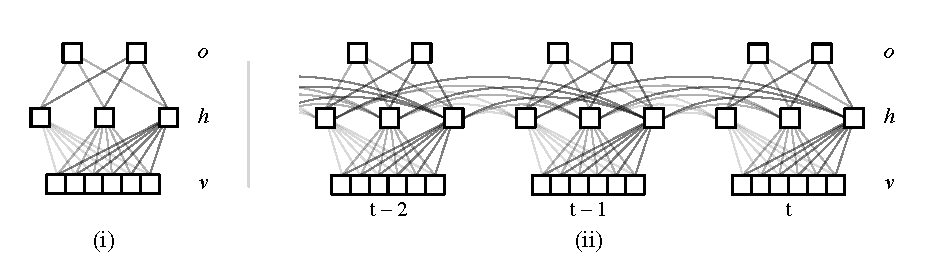
\includegraphics[width=\textwidth]{nnets}
\caption{\small{Time-Delay (i) and Recurrent (ii) multi-layer neural network architectures.}}
\label{fig:networks}
\end{figure}

Comparing the structures of Figures \ref{fig:filters} and \ref{fig:networks}, it is clear that digital filters and neural networks share similar architectures.
TDNNs are actually what is known in signal processing as an FIR filterbank, and RNNs exhibit behavior similar to IIR filters.
There are significant differences between these two alternate interpretations of digital filters and neural networks, however.
Arguably the most important discrepancy is that digital filters are classically forced to be linear, time-invariant systems, whereas neural networks embrace non-linear behavior.
While the LTI constraint makes mathematic analysis tractable, the cascade of any number of linear systems is itself a linear system, thereby limiting the kinds of functions that can be implemented by filters alone.
Leveraging data to learn the parameters of a network allows neural networks to sidestep this constraint and construct hierarchical data representations.
However, the handling of time is a relatively unsolved problem in neural network research, but time and phase are well-understood concepts in digital signal processing.
Fusing these two disconnected perspectives allows each domain to inform the other, potentially leading to the advent of information processing models better suited to making sense of time.


\section{Mathematical Formulation}
\label{sec:example}

Neural networks have achieved widespread success in a variety of computer science topics, operating on two related design principles:
one, some desired invariance is achieved through multiple non-linear processing layers;
and two, data-driven learning is able to find those parameters that yield the appropriate representations, blurring the line between feature extraction and classifier.
The key advantage of such machines here is that many design decisions affecting the input representations can be delayed until the learning stage.
Similarly, the two elements that must be addressed when using such methods is the design of the architecture and the approach used to find these parameters.


\subsection{Architectures}
\ref{subsec:architectures}

Conventionally, a neural network transforms an input $X_{1}$ into an output $Z_{L}$ via a composite nonlinear function $F(\cdot \vert \Theta)$, given a parameter set $\Theta$.
This is traditionally achieved as a cascade of $L$ simpler nonlinear functions $f_l(\cdot \vert \theta_l)$, referred to as layers, the order of which is indexed by $l$:

\begin{equation}
\label{eq:layers}
F(X_{1} \vert \Theta) = f_{L}(  ... f_2(f_1(X_{1} \vert \theta_1) \vert \theta_2) ) ... \vert \theta_{L})
\end{equation}

\noindent In this formulation, $F = [f_1, f_2, ... f_{L} ]$ is the set of layer functions, $\Theta = [\theta_1, \theta_2, ... \theta_{L} ]$ is the corresponding set of layer parameters, the output of one layer is passed as the input to the next, as $X_{l+1} = Z_{l}$, and the overall \emph{depth} of the network is given by $L$.

Importantly,

While a layer $f_l$ can be any differentiable function, we limit our focus in this work to fully-connected, or \emph{affine}, transformations, defined by the following:

\begin{equation}
\label{eq:fclayer}
f_l(X_l \vert \theta_l) = h( W \bullet X_{l} + b), \theta_l = [W, b]
\end{equation}

\noindent Here, the input $X_l$ is flattened to a column vector of length $N$ and the dot-product is computed with a weight matrix $W$ of shape $(M, N)$, followed by an additive vector bias term $b$ with length $M$.
Note that an affine layer transforms an $N$-dimensional input to an $M$-dimensional output, referred to as the \emph{width} of the layer.
The final operation is a point-wise nonlinearity, $h(\cdot)$, defined here as $tanh(\cdot)$, which is bounded on $(-1, 1)$.

When used as a classification system, the first $L-1$ layers of a neural network can be viewed as feature extractors, and the last layer, $f_L$, is a simple linear classifier.
The output representation can be made to behave like a posterior by constraining the $L_1$-norm of the output to equal $1$.
Traditionally, the probability mass function $P(\cdot)$ for an input $X_1$ is achieved by applying the softmax operation to the output of the network, $Z_L$, defined as follows:

\begin{equation}
\label{eq:softmax}
P(X_1 | \Theta) = \sigma(Z_L) = \frac{\exp(Z_{L})}{ \sum_{m=1}^{M_{L}}\exp{(Z_{L}[m])}}
\end{equation}

\noindent Again, note that $Z_{L}$ is the output of the final layer, $f_L$, and thus $M_L$ is the dimensionality of the classifier and equal to the number of classes in the problem.
Therefore, the most likely class for an observed input, $X_1$, is given by $argmax(P(X_{1} | \Theta))$.

\subsection{Energy-based Learning}

Having written the full network as a probability mass function, the network can be trained by iteratively minimizing the negative log-likelihood of the correct class for a set of $K$ observations:

\begin{equation}
\label{eq:nll}
\mathcal{L}=-\sum_{k=0}^K log(P(X^k = Y^k \vert \Theta))
\end{equation}

\noindent Expressed in this manner, $X^k$ and $Y^k$ are the input data and corresponding class label, respectively of the $k^{th}$ observation.

We can then minimize this loss function via mini-batch stochastic gradient descent.
Here, gradients are computed with $K>1$, but much smaller than the total number of observations, by sampling datapoints from the training set and averaging the loss over the batch.
Specifically, the update rule for $\Theta$ is defined as its difference with the gradient of the scalar loss $\mathcal{L}$ with respect to the parameters $\Theta$, weighted by the learning rate $\eta$, given by the following:

\begin{equation}
\label{eq:updaterule}
\Theta \leftarrow \Theta - \eta * \frac{ \delta \mathcal{L}}{\delta \Theta}
\end{equation}


\section{Recent Developments}
\label{sec:example}

Though models and architectures for neural information processing had been proposed throughout the last half of the $20^{th}$ century, there were several issues that impeded progress for decades.
Early neural networks were highly prone to overfit, producing systems that failed to give good performance on unseen data.
These issues were exacerbated by overzealous estimates of how and when ``strong'' AI could be achieved and the technological limitations of early computers.
For example, the idea of backpropagation as a learning algorithm had been presented in 1969, but the complexity of networks and number of iterations needed for convergence were computationally prohibitive for the time period \cite{}.

This remained the reality until the 1990's, when many of these barriers started to fall and neural network research could begin to recover from widespread negative opinion.
Along with advances in technology, it was discovered that stochastic gradient descent (SGD) worked as well, if not better, than exhaustive batch methods, meaning that ---keeping consistent with the previous mountain climbing analogy--- the system could take ``steps'' in the right direction faster.
As a result, the algorithm is far more efficient and therefore feasible in practice.
Additionally, a novel architecture, based on knowledge of the visual cortex and building upon the work of \cite{Fukushima1988}, known as a convolutional neural network demonstrated that these models could be successfully applied to real world problems, the first instances being signature recognition \cite{LeCun1994} and handwritten digit classification \cite{LeCun1998}.

Though this approach worked well for a few specific tasks, its applicability was limited in other domains because it required a substantial amount of labeled, ground-truth data for supervised training.
Fully supervised learning, however, is often impractical and difficult to scale to every application.
As a result, much effort was invested in finding unsupervised methods of training large networks.
Finally in 2006, one such method, called contrastive divergence was proven successful, using a slightly different processing model known as a Restricted Boltzmann machine (RBM).
The important characteristic of an RBM is that it can be used to generate, as well as process, information in both directions.
This is fundamental to contrastive divergence, which trains each layer of a deep network separately by learning to recreate its input data.
By analogy, this approach aims to discover structure in the data that occurs with high probability and effectively ``ignore'' everything else.
When strung together as a full network, these systems are referred to as deep belief networks (DBNs), as a result of their probabilistic formulation.
Subsequently, a similar model called an autoencoder \cite{Vincent2010}, or ---an alternative interpretation from another research team--- Predictive Sparse Decomposition \cite{Ranzato2007}, incorporates roughly the same principles with deterministic interpretation of these concepts.
In either view of the parameter optimization problem, learning algorithms now exist that can leverage large quantities of unlabeled data to tune large networks with minimal supervision.
These advances have collectively ushered in a new era of machine learning, referred to as \emph{deep learning}, named so for the multiple levels of information processing and the manner in which the parameters of the system are discovered from data.
Deep learning is therefore based on two principles: first, that complex problems can be decomposed into a series of simpler subproblems; and second, what exactly these simpler subproblems are or should be can be discovered from a corpus of data.

Looking closely at recent work in deep learning, most of the effort has been invested in areas of static input representations, i.e. computer vision and still images.
As evidenced by music, audio, and video, time plays an extremely important role in the way that information is conveyed.
Though CNNs have been applied to signals with a temporal dimension \cite{LeCun1994}, recursive architectures have shown promise for addressing the problem of time and sequences in data.
Initial efforts to train RNNs however, even with supervised methods, proved extremely challenging, with the observed phenomena manifesting as numerical stability issues of the gradient.
Due to the recursive nature of the model, backpropagating the error signal through time is prone to make the amplitude of the gradient either vanish or explode.
Despite these difficulties, several approaches and optimization methods have been developed in recent years that encourage further exploration of these models.

One of the earliest successful attempts to circumvent the issue of gradient stability was realized through a method called LSTM \cite{Schmidhuber1997}, where the gradient signal is ``latched'' by a hidden unit such that its information could be saved long enough to be useful.
Similar notions surround the notion of reservoir computing, such as echo-state networks, which employ feedback connections to cache arbitrary temporal information such that a second non-recursive layer ---being far easier to train--- might be able to make sense of it \cite{Jaeger2002}.
Alternatively, conditional DBNs have been employed to model, classify, and generate convincing sequences of human motion \cite{JMLR2011}, and can be thought of as a probabilistic CNN.
Recent research has found that more complex optimization methods are sufficient to train RNNs directly without changing the underlying model \cite{Martens2010}, giving encouraging qualitative results on motion \cite{Sutskever2008} and text generation \cite{Sutskever2011}.
There has also been initial work investigating discriminative recursive models that also leverage unsupervised training \cite{Rolfe2013}.
This research is particularly exciting, as it demonstrates that such models are actually within reach.
Reflecting on the corpus of deep learning work in the past decade however, it should be noted that the majority of these breakthroughs ignore audio, and even more so music, signals, focusing instead on vision or natural language processing tasks.


\section{Previous Efforts in Automatic Music Description}

This realization is beginning to spread throughout the MIR community, and there is, understandably, an increasing interest in the application of deep learning methods to these problems.
Among the first uses of deep learning were the application of CNNs to the detection of onsets \cite{Lacoste2007} and long short-term memory to model symbolic music sequences \cite{Eck2008}.
Deep Belief Networks quickly gained popularity for genre recognition \cite{Hamel2009}, mood estimation \cite{Schmidt2011}, note transcription \cite{Nam2011}, and artist recognition \cite{Dieleman2011}, but somewhat surprisingly many of these methods operate on single, short-time observations of the music signal.
Incorporating longer time-scales, CNNs have also been used to classify inputs on the order of seconds for, again, genre recognition \cite{Li2010}, instrument classification \cite{Humphrey2010} and chord estimation \cite{Humphrey2011, Humphrey2012b}.
Predictive Sparse Decomposition (PSD) and methods inspired by sparse coding have also seen a spike in activity over the last two years for a variety of tasks \cite{Henaff2011, Nam2012}, but despite being developed for deep learning, neither of these systems are actually hierarchical.

% It is worthwhile to note that many, if not all, of these works have achieved state of the art performance on their respective tasks, often in the first application of the method to the area.
% Any instances where this has occurred, however, deep learning techniques have simply been directly some kind of derived audio representation with minimal modification.
% It is therefore important to realize that these methods have never been tailored to address the nuances of music signals, and more importantly time.
% Overall, only CNNs make an effort to consider observations on the order of seconds, but do so in an admittedly awkward way, requiring the observation length be defined \emph{a priori}.
% The machine is ultimately limited to the amount of information it sees in its analysis, and there is obviously no fixed duration in which all musical behavior resides.

\section{Summary}
